\subsection{Workflow}
\label{sec:workflow}

For each code, the Autograde script does the following:

\begin{enumerate}

  \item \textbf{Pre-processing}. A user-supplied script acts on the code in any
    desired way, e.g. unzipping code, commenting out statements or extracting
    information.  This step is optional; the script may be absent.

  \item \textbf{Compilation}. Given the language option, Autograde determines
    the compiler to use and its flags, then compiles the code to produce an
    executable. For languages with interpreters, this step is omitted.

  \item \textbf{Execution}. With an optional input feed file which gives the
    input expected by the program, the code is executed.  Its output and error
    streams are captured and placed into ID-labelled files.

  \item \textbf{Post-processing}. A user-supplied script acts on any files
    generated by the compilation and execution stages. Minimally it copies the
    output and error messages into their respective directories. It may also
    extract information on certain error messages and respond by terminating.
    This step is also optional and the script may be absent.

  \item \textbf{Auto-evaluation}.  The Autograde script calls the Java
    auto-evaluation program, passing to it the requisite information, i.e.  the
    locations of grading specification and source files. 

  \item \textbf{Profiling}.  In tandem with compilation, execution, and
    auto-evaluation, the script logs errors to a file for processing
    by a profiling module.

\end{enumerate}

Depicted in Fig.\ref{fig:workflow} is the workflow of the system.

\begin{figure}
  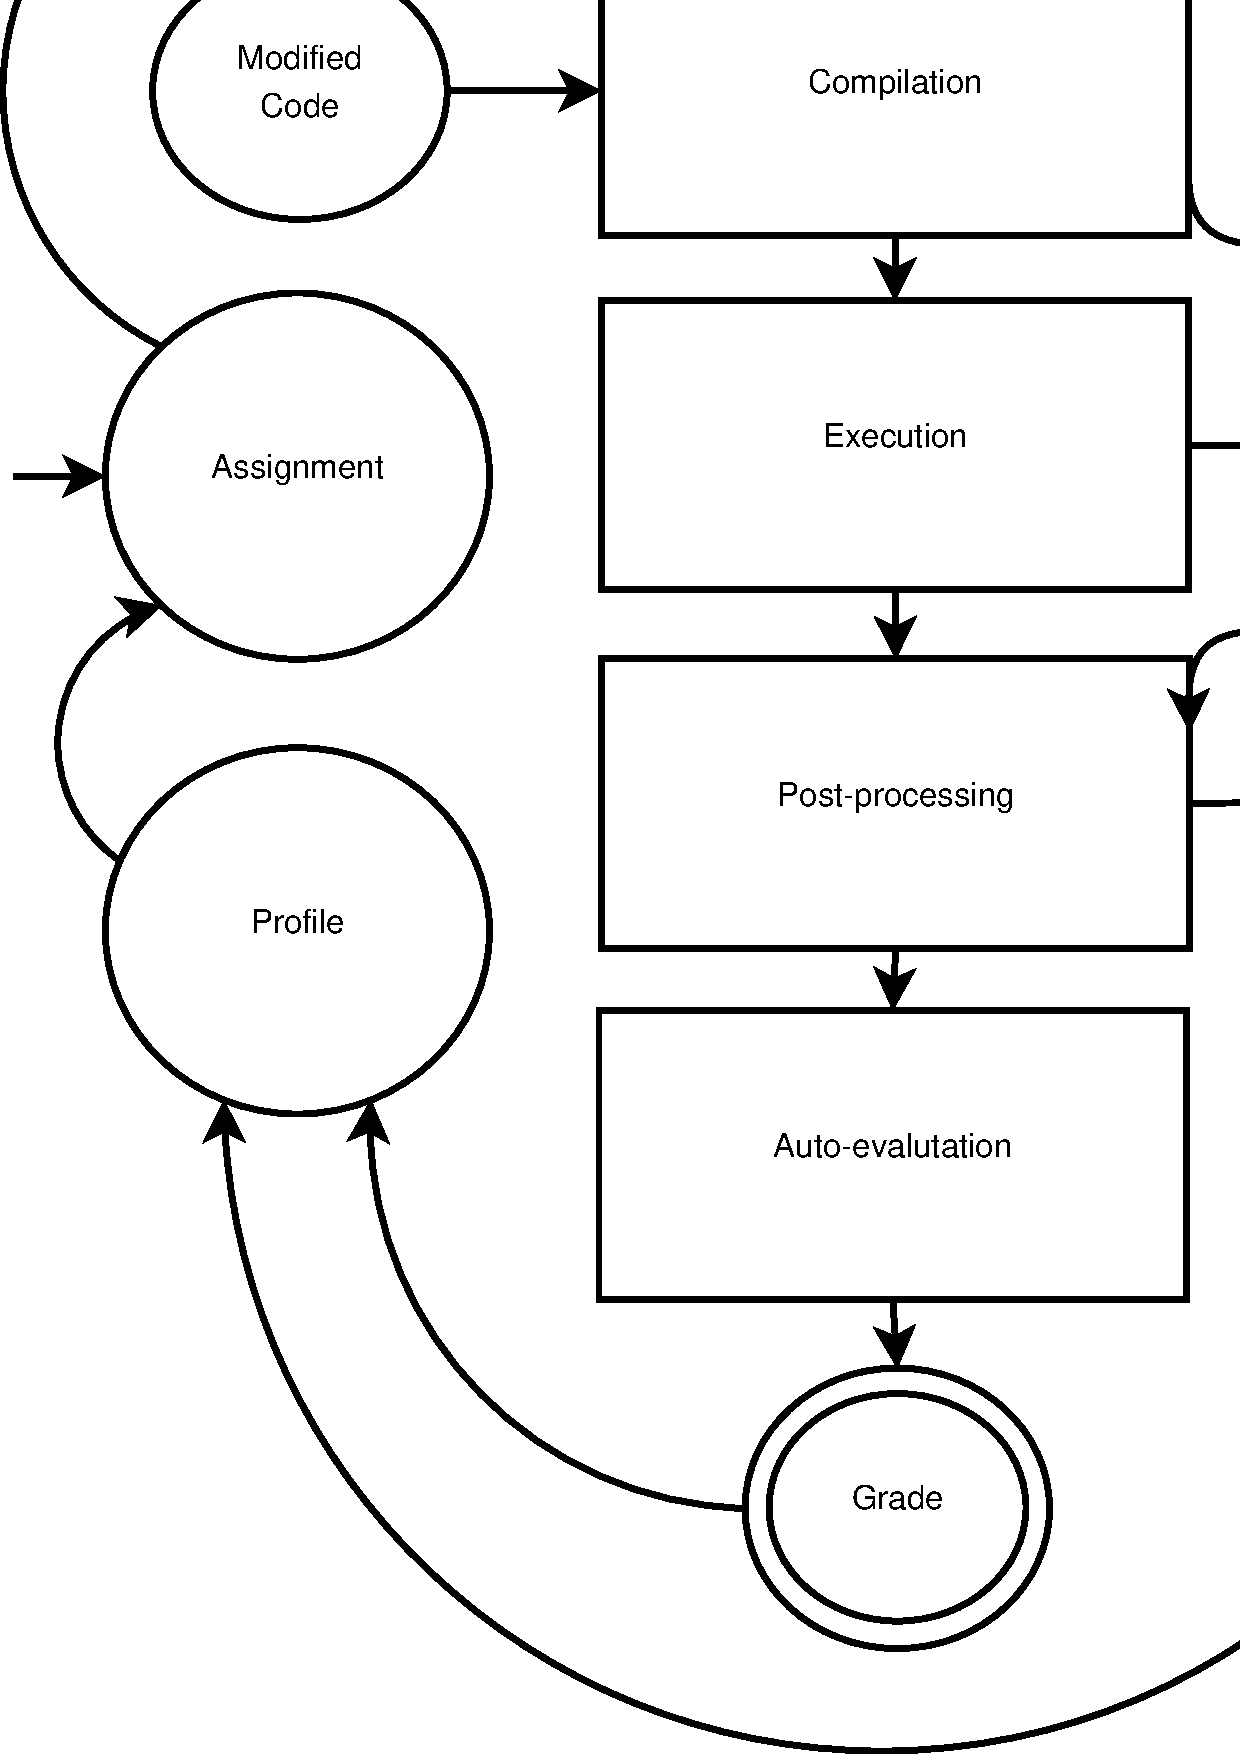
\includegraphics[width=.45\textwidth]{figs/workflow.pdf}
  \caption{The workflow of the system begins with an assignment specification,
following the steps of the Autograde batch processor to produce a grade and
profile, which is subsequently used to generate future assignment
specifications.}
  \label{fig:workflow}
\end{figure}


